\documentclass[a4paper]{article}
\usepackage[14pt]{extsizes} % для того чтобы задать нестандартный 14-ый размер шрифта
\usepackage{amsmath}
\usepackage[unicode, pdftex]{hyperref}
\usepackage[usenames]{color}
\usepackage[warn]{mathtext}
\usepackage[T2A]{fontenc}
\usepackage[utf8]{inputenc}
\usepackage[english, russian]{babel}
\usepackage{amsfonts}
\usepackage[left=20mm, top=15mm, right=15mm, bottom=15mm, nohead, footskip=10mm]{geometry} % настройки полей документа
\usepackage{graphicx}
\usepackage{wrapfig}
\usepackage{placeins}
\usepackage{float}
\begin{document}
\author{Горяной Егор}
\date{28 мая 2022}
\title{Дифракция на CD-диске}
\maketitle


\section{Теоретическая часть}
{Для того, чтобы записывать информацию на CD-диск, в нём делают специальный углубления --- питы. Каждый пит имеет примерно 100 нм в глубину и 500 нм в ширину. Длина пита варьируется от 850 нм до 3,5 мкм. Шаг дорожек в спирали составляет 1,6 мкм. Питы рассеивают или поглощают падающий на них свет, а подложка — отражает. Поэтому записанный компакт-диск — пример отражательной дифракционной решётки с периодом порядка нескольких микрон.}
\begin{figure}[H]
    \centering
    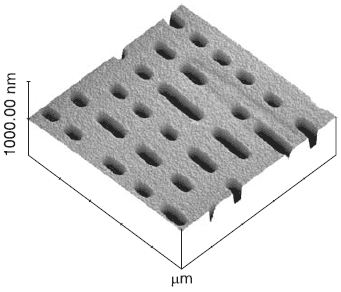
\includegraphics[scale=1]{cd_disk.png}
    \caption{CD-диск под микросопом}
\end{figure}
Уравнение решётки в случае нормального падения света:
\begin{equation}\label{eq1}
d\sin\theta_m=m\lambda
\end{equation}
Пусть свет падает нормально в точку, находящуюся на расстоянии $R$ от центра диска. Тогда: расстоянию $d$ соответствует какой-то угол $\Delta\varphi$.\\
\\
При этом имеем равенство: $\Delta\varphi=\displaystyle\frac{d}{R}$.\\
\\
Поскольку период решётки $d$ одного порядка с длиной пита $b$, то можно сказать, что:
\begin{equation}\label{eq2}
\displaystyle\sum\limits_{i=1}^{N}\Delta\varphi_i\approx\pi
\end{equation}
\\
С другой стороны:
\begin{equation}\label{eq3}
\sum\limits_{i=1}^{N}\Delta\varphi_i=\sum\limits_{i=1}^{N}\displaystyle\frac{d}{R} = N \displaystyle \frac {d}{R}
\end{equation}
\\
Приравнивая (2) и (3), получим:
\begin{equation}\label{eq4}
N=\displaystyle\frac{\pi R}{d}
\end{equation}
\\
При этом разрешающая способность решётки:
\begin{equation}\label{eq5}
R=mN=\displaystyle\frac{\lambda}{\delta\lambda}
\end{equation}
\\
Подставим $m=1,$ (1) и (4) в (5) и выразим $\delta\lambda$:
\begin{equation}\label{eq6}
\delta\lambda=\displaystyle\frac{\lambda^2}{\pi R\sin\theta_1}
\end{equation}
\\
\section{Практическая часть}
\end{document}


